\section{实验设计}
\subsection{程序计数器(PC)}\label{sub:PC}
\subsubsection{功能描述}
d触发器结构,用于储存 PC(一个周期)
\subsubsection{接口定义}
\begin{table}[htp]
	\caption{PC接口定义}\label{tab:pcdef}
	\begin{center}
		\begin{tabular}{|l|l|l|p{6cm}|}
		\hline
		\textbf{信号名} & \textbf{方向} & \textbf{位宽} & \textbf{功能描述}\\ \hline \hline
		clk     & in    & 1     & 时钟周期\\ 
		rst     & in    & 1     & 复位信号\\ 
		newpc   & in    & 32    & 新地址\\ 
		pc      & out   & 32    & 输出的地址\\ 
		Inst\_ce & out  & 1     & 判断是否pc发生改变\\ 
		\hline
		\end{tabular}
	\end{center}
	\end{table}
\subsubsection{逻辑控制}
根据rst是否为1给pc和inst\_ce赋值。当为1时,pc不变,inst\_ce为0,rst为0,pc改变,inst\_ce为1。
\subsection{加法器(Adder)}\label{sub:adder}
\subsubsection{功能描述}
用于计算下一条指令地址。
\subsubsection{接口定义}
\begin{table}[htp]
	\caption{Adder接口定义}\label{tab:adderdef}
	\begin{center}
		\begin{tabular}{|l|l|l|p{6cm}|}
		\hline
		\textbf{信号名} & \textbf{方向} & \textbf{位宽} & \textbf{功能描述}\\ \hline \hline
		Pc          & in    & 32    & 初始位置\\ 
		Pc\_next    & out   & 32    & 之后的位置\\ 
		clk         & in    & 1     & 时钟周期\\ 
		rst         & in    & 1     & 复位信号\\ 
		Inst\_ce    & in    & 1     & Pc部分的pc是否变换\\ 
		\hline
		\end{tabular}
	\end{center}
	\end{table}
\subsubsection{逻辑控制}
和上文的pc相结合,最后达成目的。
\subsection{控制器(Controller)}\label{sub:controller}
\subsubsection{功能描述}
对于(a)main\_decoder:负责判断指令类型,并生成相应的控制信号。

对于(b)alu\_decoder:负责 ALU 模块控制信号的译码。
\subsubsection{接口定义}
\begin{table}[htp]
	\caption{main\_decoder接口定义}\label{tab:maindecoderdef}
	\begin{center}
		\begin{tabular}{|l|l|l|p{6cm}|}
		\hline
		\textbf{信号名} & \textbf{方向} & \textbf{位宽} & \textbf{功能描述}\\ \hline \hline
		op         & in    & 6     & 指令\\ \hline
		memtoreg   & out   & 1     & 回写的数据来自于ALU计算的结果/存储器存储的数据\\ \hline
		memwrite   & out   & 1     & 是否要书写数据存储器\\ \hline
		branch     & out   & 1     & 是否为branch指令且满足branch的条件\\ \hline
		regwrite   & out   & 1     & 是否书写寄存器堆\\ \hline
		jump       & out   & 1     & 跳转\\ \hline
		aluop      & out   & 2     & ALU选择\\ 
		\hline
		\end{tabular}
	\end{center}
	\end{table}
	
\begin{table}[htp]
	\caption{alu\_decoder接口定义}\label{tab:aludecoderdef}
	\begin{center}
		\begin{tabular}{|l|l|l|p{6cm}|}
		\hline
		\textbf{信号名} & \textbf{方向} & \textbf{宽度} & \textbf{含义}\\ \hline \hline
		funct & in & 6 & 指令功能码 \\ 
		aluop & in & 2 & 算术逻辑单元操作码 \\ 
		alucontrol & out & 3 & 算术逻辑单元控制信号(指令的最终结果) \\ 
		\hline
		\end{tabular}
	\end{center}
	\end{table}
		
\subsubsection{逻辑控制}
对于(a)main\_decoder:控制器输出的控制信号,用于控制器件的使能和多路选择器的选择,因此,根据 
不同指令的功能分析其所需要的路径,即可得到信号所对应的值。

对于(b)alu\_decoder:先根据aluop判断是否为sw和beq,其他的操作要根据funct进一步判断,在这里用了三目操作符的方式。
同时最后假如funct的数据不对,alucontrol=000不做任何操作。
\subsection{存储器(Block Memory)}\label{sub:ctl}
用于在 FPGA 中高效地存储和访问指令数据。
\subsubsection{存储器Basic界面}
\begin{figure}[htbp]
    \centering
    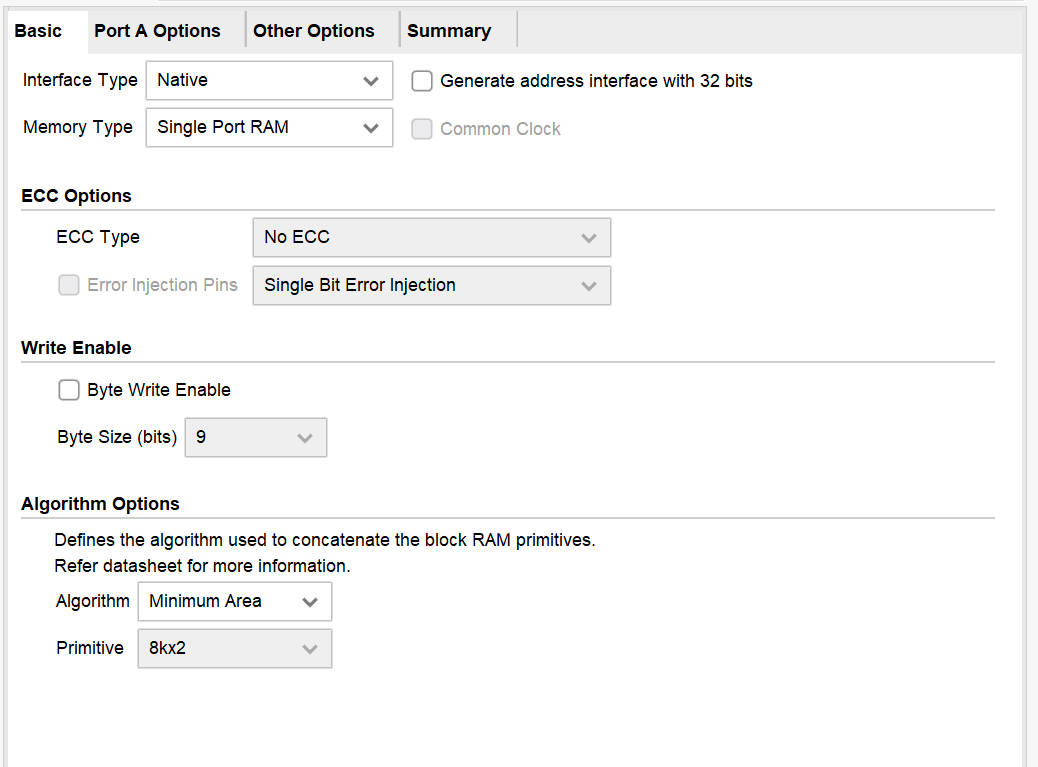
\includegraphics[width=0.8\textwidth,height=6in,keepaspectratio]{BMG1.jpg}
    \caption{存储器Basic界面}
    \label{image1}
\end{figure}
\subsubsection{存储器Part A Options界面}
\begin{figure}[htbp]
    \centering
    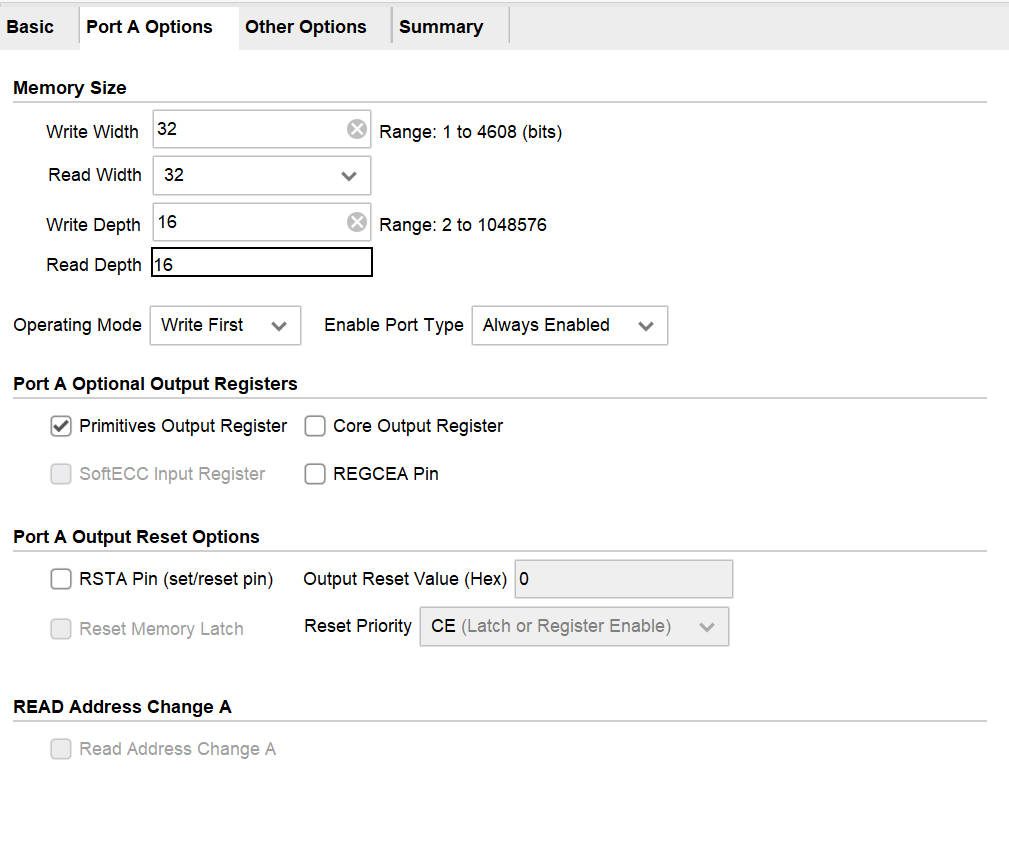
\includegraphics[width=0.8\textwidth,height=6in,keepaspectratio]{BMG2.jpg}
    \caption{存储器Part A Options界面}
    \label{image2}
\end{figure}
\subsubsection{存储器Other Options界面}
\begin{figure}[htbp]
    \centering
    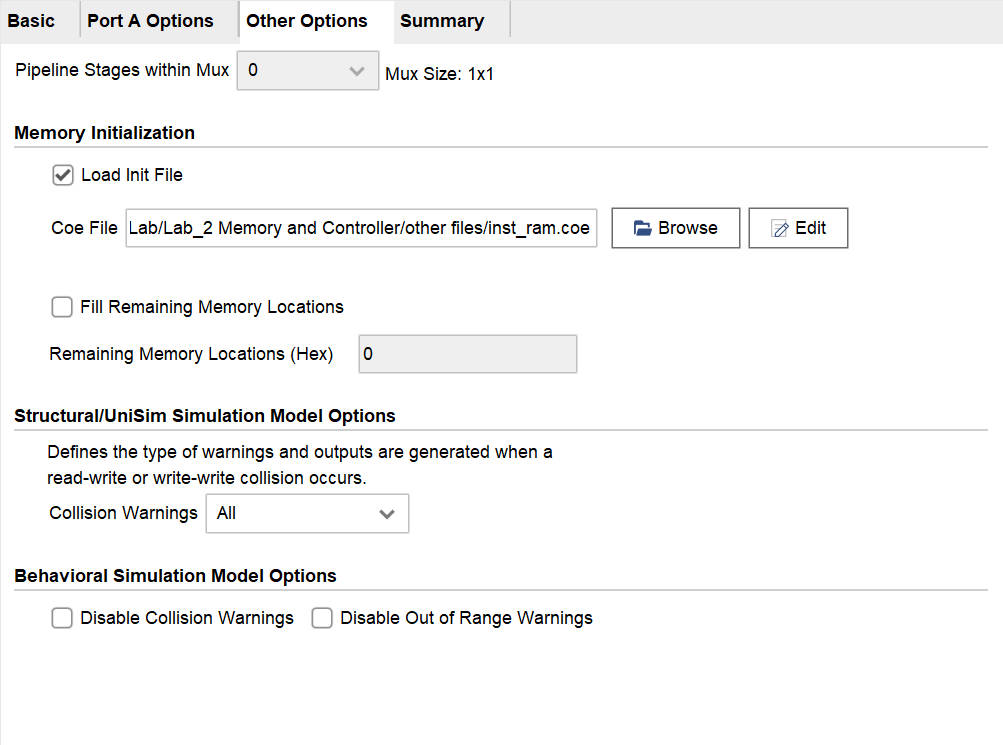
\includegraphics[width=0.8\textwidth,height=6in,keepaspectratio]{BMG3.jpg}
    \caption{存储器Other Options界面}
    \label{image3}
\end{figure}